\documentclass{article}

\usepackage{graphicx}
\usepackage{hyperref}
\usepackage{xcolor}
\usepackage{listings}
\lstloadlanguages{C++,bash}
\lstset{basicstyle=\ttfamily,
  emphstyle=\underbar,
  language=C++
}

\newcommand{\code}[1]{\lstinline!#1!}
\newcommand{\fn}[1]{\texttt{#1}}

\title{Morton order matrices in C++}
\author{Rupert Nash \\ \url{r.nash@epcc.ed.ac.uk}}

\begin{document}
\maketitle{}

Source for this can be obtained from Github. Get a new copy with:
\begin{lstlisting}[language=bash]
git clone https://github.com/rupertnash/cpp4computsci
\end{lstlisting}
or update your existing one with
\begin{lstlisting}[language=bash]
git pull
\end{lstlisting}
then you can 
\begin{lstlisting}[language=bash]
cd cpp4computsci/practicals/02
\end{lstlisting}


The Morton ordering (or z-ordering) of a matrix lays out the elements
along a recursive z-shaped curve, as shown in
\autoref{fig:morton}. You can compute the Morton index \code{z} from
the $x$ and $y$ indices (\code{i} and \code{j} respectively) by
interleaving their bits. An example is shown in
\autoref{tab:morton}.

\begin{figure}[htb]
  \begin{center}
    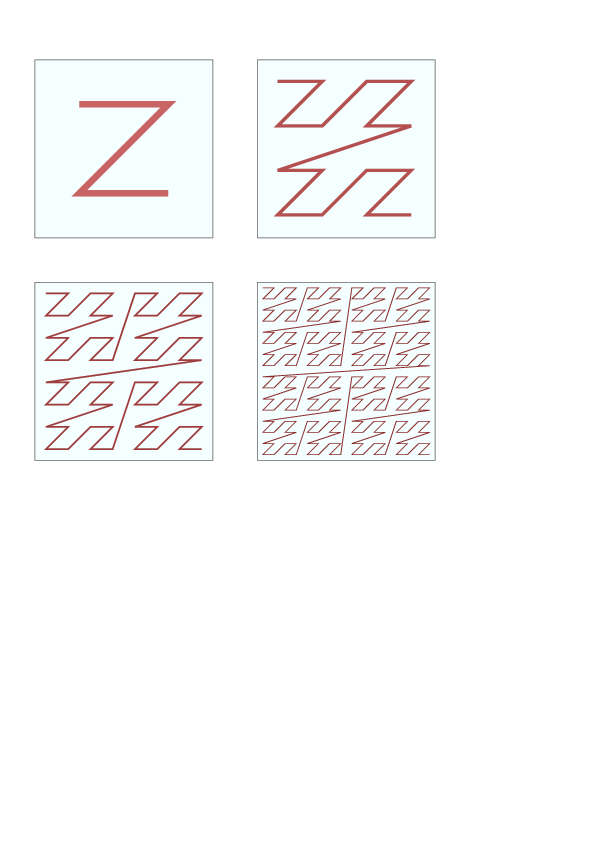
\includegraphics[width=0.5\textwidth]{mortonorder}
    \caption{Four iterations of the Z-order curve. (From
      \href{https://en.wikipedia.org/wiki/Z-order_curve}{Wikipedia})}
    \label{fig:morton}
  \end{center}
\end{figure}
\clearpage
\begin{table}[htb]
  \begin{tabular}{l|rrrr}
    &    0 &  1 &  2 &  3 \\
    \hline
    0 & 0 & 1 & 4 & 6 \\
    1 & 2 & 3 & 5 & 7 \\
    2 & 8 & 9 & 12 & 13 \\
    3 & 10 & 11 & 14 & 15 \\
  \end{tabular}\quad
  \begin{tabular}{l|rrrr}
    &   00 & 01 & 10 & 11 \\
    \hline
    00 & 0000 & 0001 & 0100 & 0101 \\
    01 & 0010 & 0011 & 0110 & 0111 \\
    10 & 1000 & 1001 & 1100 & 1101 \\
    11 & 1010 & 1011 & 1110 & 1111 \\
  \end{tabular}
  \caption{Mapping between $x-y$ indexes and Morton index for a matrix
    of size $4\times 4$. Decimal on the left and binary on the right.}
  \label{tab:morton}
\end{table}


The advantage of laying out data in this way is that it improves data
locality (and hence cache use) without having to tune a block size or
similar parameter. On a modern multilevel cache machine\footnote{An
  ARCHER node has L1, L2, and L3 caches, and the RAM is divided into
  two NUMA regions. If using co-arrays or OpenSHMEM one can view local
  RAM as a cache for the distributed memory - i.e. 6 levels!}, this
means it can take good advantage of all the levels without tuning
multiple parameters.

This exercise will walk you through a simple implementation.

I have included implementations of the functions that do the
``bit-twiddling'' for translating between a two-dimensional $x$-$y$
index and the Morton index, in the file \verb!bits.hpp!. These are
reasonably fast, but can be beaten if you are interested to try! 

In what follows each section corresponds to a subdirectory with the
same number.

\section{Implement the underlying data storage and element access}
Go to the step 1 directory:
\begin{lstlisting}[language=bash]
cd cpp4computsci/practicals/02/step1
\end{lstlisting}

Using the partial implemenation in \verb!matrix.hpp!, your task is to
implement the allocation (and release!) of memory to store the data
and to use the helper functions from \verb!bits.hpp! to allow element
access. You will need to implement a number of member functions
(marked in the source with \code{\\\\ TODO}) and add whatever data
members are needed (marked in the same way).

There is a test program \verb!test_matrix_basic.cpp! which runs a few
sanity checks on your implementation (and similarly with
\verb!test_bits.cpp!). The supplied \verb!Makefile! should work.

\section{Implement a basic iterator to traverse the matrix in order}

Go to the step 2 directory:
\begin{lstlisting}[language=bash]
cd cpp4computsci/practicals/02/step2
\end{lstlisting}

I have a potential solution to part 1 here, but feel free to copy
your implementation into this. 

The exercise here is to complete the \code{matrix_iterator} class
template that I have started. I've provided most of the boilerplate to
have this work as a ``bidirectional iterator''.  See
\url{http://en.cppreference.com/w/cpp/concept/BidirectionalIterator}
for full details of what this means, but basically it's one that can
move forward and backward through the data.

Again, the things that need added are marked with \code{\\\\
  TODO}). The most important thing to think about is how you will
refer to the current position and be able to traverse through it
efficiently in Morton order - the performance should be identical to
looping over a raw pointer!


\end{document}
